\documentclass[a4paper]{article}
\usepackage[utf8]{inputenc}
\usepackage[english]{babel}
\usepackage{moreverb}
\usepackage{graphicx}
\title{Project Report \\ EDA216 Database Technology \\ Krusty Kookies AB}
\date{\today}
\author{Fredrik Paulsson \\ dat11fp1@student.lu.se \and Jonas Jacobsson \\ dat11jja@student.lu.se}
%\setcounter{secnumdepth}{5}
%\setcounter{tocdepth}{5}
\begin{document}
\maketitle
%\tableofcontents
\newpage

%Report
%The report should be written in English (you may write in Swedish if you absolutely cannot produce readable English). Contents:
%2
%1. A cover sheet with the name of the project, your names, education programs, and e-mail addresses. You must check mail to these addresses regularly.
%Also give the date of submission and complete instructions for running your program.
%2. An introduction (what the project is about, etc.).
%3. Something about requirements that you fulfill or don’t fulfill.
%4. An outline of your system (which database manager you use, which programs you have
%written, how the programs communicate with the database, etc.).
%5. An E/R diagram which describes the system.
%6. Relations. Indicate primary keys, possibly secondary keys, and foreign keys. You must
%show that the relations are normalized according to your chosen normal form (if a relation “obviously” is in BCNF you may say so, provided that you justify your statement). If a
%relation is in a lower normal form than BCNF, you must justify this choice.
%7. SQL statements to create all tables, views, stored procedures, and other database elements.
%(Don’t include statements to create the initial contents of the database.)
%8. A user’s manual (not necessary if everything in the program is self-explanatory).

\section{Introduction}
In this project we were to develop a database system that handles production, orders and deliveries of cookies in the company Krusty Kookies Sweden AB. In order to develop the database system we have to produce an E/R model of the database, create relations corresponding to the E/R model and finally implement those relations in a database management system. In the project we also had to implement a client program that interfaces to our database. This client program only handles production of cookies and blocking of pallets.

This report serves as documentation of our implementation. 

\section{Requirements}

\section{System Outline}
Our system uses MySQL as the database management system and our client interface is written in PHP for optimal portability.

\begin{description}

\end{description}
\section{E/R Model}
\begin{figure}[!h]
\centering
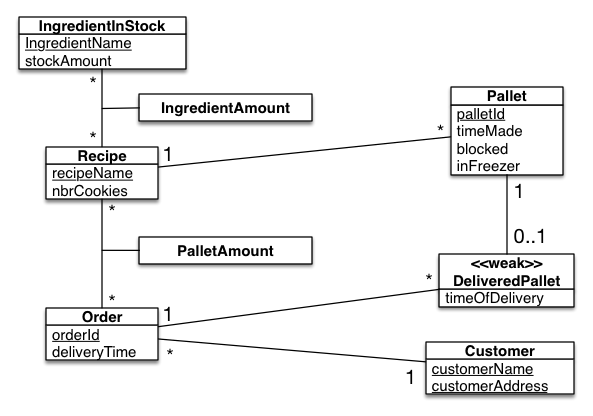
\includegraphics[scale=0.7]{projectUMLFinal.png}
\caption{UML diagram for the E/R model.}
\label{uml}
\end{figure}

\section{Relations}

\texttt{IngredientsInStock(\underline{ingredientName},stockAmount)} \\
\texttt{Recipes(\underline{recipeName},nbrCookies)} \\
\texttt{IngredientsInRecipe(\underline{\textit{ingredientName},\textit{recipeName}},ingredientAmount)} \\
\texttt{Customers(\underline{customerName,customerAddress})} \\
\texttt{Orders(\underline{orderId},deliveryTime,\textit{customerName,customerAddress})} \\
\texttt{RecipesInOrders(\underline{\textit{recipeName},\textit{orderId}},palletAmount)} \\
\texttt{Pallets(\underline{palletId},timeMade,blocked,inFreezer,\textit{recipeName})} \\
\texttt{DeliveredPallets(\underline{\textit{palletId}},timeOfDelivery,\textit{orderId})}


\section{SQL Statements}


\section{User Manual}
%\begin{thebibliography}{1}
%\bibitem{wikipedia}
%http://en.wikipedia.org
%\end{thebibliography}
\end{document}